\documentclass{article}
\usepackage[utf8]{inputenc}
\usepackage{amsfonts}
\usepackage{amsmath}
\usepackage{hyperref}
\usepackage{graphicx}
\usepackage[export]{adjustbox}
\usepackage{xcolor}
\usepackage{caption}
\captionsetup[figure]{name=Slika}

\title{Projekt pri Matematiki z računalnikom: 2048}
\author{Maj Gaberšček}
\date{Ljubljana, april 2022}

\begin{document}

\maketitle

\section{Uvod}
Pri predmetu Matematika z računalnikom si je vsak študent izbral svoj projekt med številnimi, ki so vključevali projekte raznih industrijskih panog, projekte iz optimizacije, teorije iger,... Moj projekt je imel naslov \emph{Games 3: 2048}. V sklopu projekta sem si zastavil nalogo, da uspešno zasnujem uporabniški vmesnik za igranje igre 2048. Ta bo uporabniku omogočal, da sam odigra igro, ali pa izbere računalniški algoritem, ki nato sam odigra igro. Mogoča je tudi kombinacija: igralec odigra igro do neke poteze in najprej računalnik, ali obratno. Za implementacijo sem si izbral programski jezik \texttt{Java}, ki s knjižnico \texttt{Swing} omogoča relativno preprosto implementacijo uporabniškega vmesnika. Projekt sem sproti objavljal tudi na repozitorij na \texttt{Github}.

\section{Predstavitev igre 2048}

\subsection{Predstavitev}

2048 je enoigralska video igra, ki jo je izumil italijanski razvijalec Gabriele Cirulli leta 2048 in jo objavil na \texttt{Github}. Cilj igre je skupaj sestavljati različne številke na mreži in doseči število 2048. Mreža je praviloma velikosti 4x4, čeprav se v različnih variantah igre pojavlja tudi v drugih velikostih (na primer 3x3 ali 5x5).

\subsection{Pravila}

Uporabnik lahko, ko je na vrsti, naredi potezo, pri čemer ima ponavadi na voljo 4 različne: premik gor, premik dol, premik levo in premik desno. Ob premiku v želeno smer se vsako število premakne najdlje možno v tisto smer, dokler ni zaustavljena s koncem mreže ali z drugo številko. Pri tem se, če se zaletita dve enaki števili, združita v novo število, ki je vsota obeh (dvakratnik). Pri tem moramo upoštevati, da se, v kolikor se zaletijo tri enaka števila, v dvakratnih združita samo tisti dve, ki sta najdlje v smeri premika. Premika, ki mreže ne spremeni (torej ostane enaka kot pred premikom), ne smemo odigrati.

Po vsakem premiku se na naključno prazno mesto na mreži pojavi novo število, ki je 2 z verjetnostjo 90\% in 4 z verjetnostjo 10\%.

Igra je izgubljena, ko uporabnik nima več možnih potez, torej nobena poteza ne spremeni mreže. Če uporabnik doseže število 2048, je igro premagal. Večina aplikacij sicer uporabniku omogoča igranje naprej po zmagi, z ustrezno strategijo je namreč igro precej preprosto premagati.

\subsection{Točkovanje}

Igra ponuja tudi točkovanje. Po zmagi je namreč cilj uporabnikov to, da dosežejo čim več točk.

Točke se zbirajo tako, da vsakič, ko se dve števili združita v njuno vsoto, se le-ta prišteje točkam.

\subsection{Strategija človeka}

Ljudje, ki igro igrajo, ponavadi uporabijo strategijo, da največje število na mreži hranijo v določenem kotu, zraven nje pa ostala velika števila, pri čemer je cilj predvsem v tem, da največje število ne skoči iz kota.

Potrebno je tudi poudariti, da igre seveda ni mogoče igrati v nedogled. Največje število, ki ga lahko z idealno igro in precej sreče (teoretično) dosežemo, je 131072.

\section{Načrt dela}

Najprej sem v programskem jeziku \texttt{Java} ustvaril razred \texttt{Game.java}, ki predstavlja igro. Na razredu sem implementiral metode, ki služijo premikom, pojavitvam novih števil.

Nato sem s pomočjo knjižnice \texttt{Swing} definiral dva nova razreda. Razred \texttt{Panel.java}, nekakšno platno, ki služi za risanje igre in podpira interakcijo uporabnika s tipkami (premiki na igri) in razred \texttt{Frame.java}, okno, ki vsebuje platno. Okno vsebuje tudi menijsko vrstico, s pomočjo katere izbiramo nastavitve igre in igralce.

Zadnji korak je vključeval zasnovo algoritmov, ki bodo (uspešno) reševali igro in implementacija delovanja algoritmov na igri. Algoritmi so predstavljeni kot metode na razredu \texttt{Game.java}, pri čemer klic metode odigra potezo, ki jo posamezen algoritem izbere. Algoritmi so različno uspešni, predvsem pa velja pravilo, da je uspešnost algoritmov ponavadi obratno sorazmerna s časom na potezo. 

\section{Uporabniški vmesnik}

\begin{figure}[ht!]
\centering
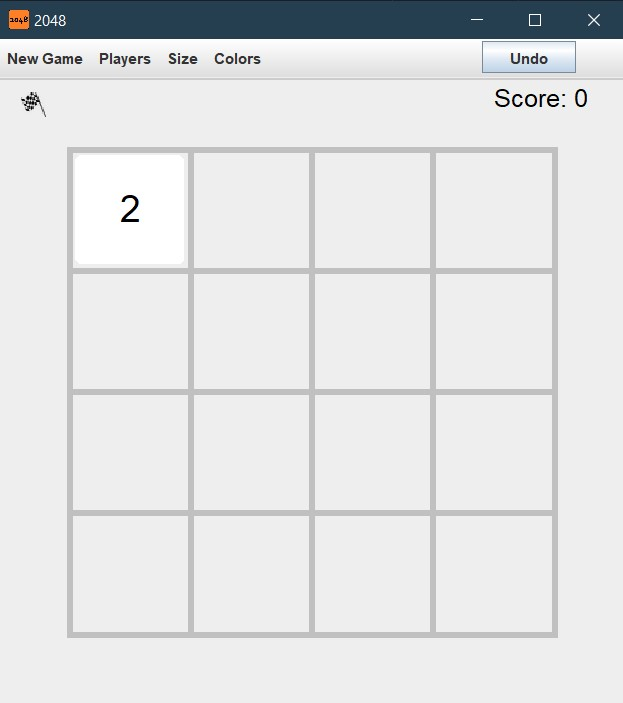
\includegraphics[width=8cm]{ui.jpg}
\caption{Posnetek zaslona uporabniškega vmesnika, ko aplikacijo zaženemo}
\label{ui}
\end{figure}

Na Sliki \ref{ui} je posnetek zaslona uporabniškega vmesnika aplikacije. Kot lahko vidimo, se čez večino okna nariše mreža (v primeru klasične igre 4x4). Vsakič, ko aplikacijo zaženemo, se privzeto pojavi nova igra velikosti 4x4, ki jo lahko igramo. 

Zgoraj desno imamo napis \emph{Score}, ki nam sporoča trenutno število točk, ki smo jih dosegli. Zgoraj levo je ikonica, ki nam sporoča, kateri način igre trenutno igramo. V aplikacijo sem sprogramiral dva načina igranja: \emph{Classic}, kar pomeni da se igra konča, ko dosežemo število 2048, ter \emph{Endless}, ki omogoča igranje, dokler ne izgubimo. Način igranja izberemo v menijski vrstici, pod zavihkom \emph{New Game}.

V menijski vrstici lahko pod zavihkom \emph{Players} izbiramo igralca. Izberemo lahko igralca \emph{Player} in potem igro igramo sami, ali pa izberemo igralca \emph{Computer}. V slednjem primeru bo izbrani računalniški algoritem (ki ga izberemo pod zavihkom \emph{Computer Algorithm}) poskušal odigrati igro. Če želimo med igro spremeniti igralca, samo izberemo drugega igralca v tem podmeniju. Na primer, aplikacija omogoča, da računalnik odigra do neke poteze in potem naprej odigramo mi ali obratno.

V zavihku \emph{Size} v menijski vrstici izbiramo velikost mreže igre. Pri tem je potrebno paziti, saj vsaka sprememba rezultira v novi igri (staro igro izgubimo). Implemenirane so velikosti igre 3x3, 4x4, 5x5, 6x6 in 8x8.

Zavihek \emph{Colors} nam omogoča, da si izberemo barvno shemo, ki spremeni barve. Barvne sheme lahko menjamo med igranjem, brez da to vpliva na igro.

Desno od menijske vrstice je še gumb z napisom \emph{Undo}, ki služi razveljavitvi poteze. Medtem, ko igra računalnik, gumb ne deluje. Prav tako med igranjem računalnika tudi ne delujejo tipke, ki odigravajo človekove poteze (w, a, s in d). Zavedam se, da gumb \emph{Undo} lahko uporabljamo za goljufanje igre (manipuliramo kje na mreži se bo pojavila nova številka). Vseeno je tak gumb koristen, če na primer odigramo potezo, ki je nismo želeli odigrati.

Okno z igro je spremenjive velikosti, vendar igra 4x4 najlepše izgleda v privzeti velikosti. Če okno preveč pomanjšamo, bodo številke postale prevelike za prikaz na mreži in se jih ne bo videlo.

\section{Računalnikovi algoritmi}

Implementiral sem štiri različne računalnikove algoritme za reševanje igre, ki so med seboj različno uspešni.

\subsection{Algoritem \texttt{Random moves}}

Kot nam že ime samo po sebi pove, ta algoritem uporablja naključne poteze za reševanje igre. Algoritem sam po sebi ni pretirano uspešen, je pa podlaga za bolj uspešna in kompleksna algoritma, opisana v naslednjih dveh podpoglavjih.

\subsection{Algoritem \texttt{Simulator(k)}}

Ta algoritem je v teoriji iger znan kot \emph{Pure Monte Carlo game search}. Algoritem sprejme naravno število $k$. Nato določi vse možne poteze, ki jih v dani poziciji na mreži lahko odigra. Za vsako izmed teh nato v ozadju odigra $k$ naključnih iger, kjer najprej odigra izbrano potezo, nato pa dokonča igro z algoritmom \emph{Random moves}, ki je opisan v prejšnjem podpoglavju, dokler ne izgubi. Nato primerja igre različnih potez in izbere tisto potezo, katere igre (simulacije) so v povprečju dosegle največje število točk, preden so izgubile.

Na primer, v dani poziciji sta možni potezi \emph{Premik gor} in \emph{Premik desno}. Recimo, da uporabimo število $k=10$. Algoritem v ozadju ustvari 10 kopij igre in na vsaki od njih najprej odigra potezo \emph{Premik gor}. Nato vse igre dokonča z algoritmom \emph{Random moves}. Algoritem v neko spremenjivko shrani povprečno število točk, ki jih je dosegel pri teh 10 igrah. Nato postopek ponovi za potezo \emph{Premik desno}. Ustvari 10 kopij originalne igre in na njih odigra \emph{Premik desno}, ter jih dokonča z naključnimi potezami, dokler ne izgubi vsake. Spet si v drugo spremenljivko shrani povprečno število točk na teh 10 igrah. Nato primerja povprečno število točk za potezo \emph{Premik gor} in \emph{Premik desno}. Odigra tisto, ki je v povprečju dosegla več točk.

\subsection{Algoritem \texttt{Dynamic simulator}}

\section{Analiza uspešnosti}

\section{Posnetki zaslona}

\section{Zaključek}

\section{Viri in literatura}
\begin{itemize}
    \item https://en.wikipedia.org/wiki/2048_(video_game)
\end{itemize}

\end{document}
